\documentclass[12pt, a4paper]{article}
\usepackage{import}

\usepackage{graphicx}
\usepackage{amssymb}
\usepackage{mathtools}  
\usepackage{amsthm}  
\usepackage{graphicx}
\usepackage{float}
\usepackage{caption}
\usepackage{enumerate}

\import{../../lib/}{bridge.sty}

\title{Żaczek 25.09.24}
\author{Krysia \& Bartek}
\begin{document}
\maketitle

\section*{Rozdanie 1}

\handdiagramv
{\vhand{876}{A2}{A752}{J742}}
{\vhand{AQ43}{KQJT4}{Q}{K83}}
{\vhand{KJ5}{987653}{3}{Q65}}
{\vhand{T92}{--}{KJT9864}{AT9}}{}

\begin{table}[h!]
    \centering
    \begin{tabular}{cccc}
        \nvul{W} (K) & \nvul{N} & \nvul {E} (B) & \nvul{S} \\
        -- & \pass & 1\hearts & \pass \\
        \alrts{1\nt} & \pass & \alrts{2\clubs} & \pass \\
        \alrts{2\diams} & \pass & 2\spades & \pass \\
        \alrts{2\ntx} & \pass & \alrts{3\ntx} & all \pass \\
    \end{tabular}
\end{table}

[KG] Zamiast odzywki 2\nt lepsze byłoby 3\diams. 2\nt było pytaniem o skład,
3\nt pokazało 54 i krótkość karo. Wist 7\spades do damy i króla,
walet pik zabity asem. Wyszłam w karo obawiając się jedynie odwrotu w
trefla, który zabrałby mi dojście do lew kierowych i na koniec oddałabym trefla (=).
Odwrót nastąpił w pika i reszta lew była moja (+2), a obrońcy nie wzięli nawet na asa kier.

[KK] Gadaliśmy o tym rozdaniu.\\
W sytuacji, gdy mamy do dyspozycji pytanie i 
zalicytowanie naturalnie koloru musimy zdecydować, 
która informacja jest ważniejsza. 
Mamy skład 3=0=7=3, partner nigdy tego u nas nie 
założy. 7330 jest dużo ciekawszym układem niż 
cokolwiek co partner ma do zaoferowania po 
pokazaniu już 9 kart. Do tego mamy rękę dobrą 
do gry kolorowej, znamy jego skład, ale nie 
wiemy co zrobić. \xspades AKxx \xhearts AQJxx 
\xdiams Qx \xclubs xx, 
5\diams jest świetne, a 3\nt w najlepszym razie średnie. 
Musimy nawiązać współpracę, a nie przejmować 
inicjatywę pytaniami o skład. Po naszym pytaniu 
już prowadzimy całą licytację. Akurat pełny sukces, 
po naszym 3\diams partner i tak dałby 3\nt.\\
Obrona była bardzo ciekawa, dobrze wykorzystany 
błąd przeciwników.

\pagebreak
\section*{Rozdanie 2}
\handdiagramv
{\vhand{632}{A765}{Q9}{AK32}}
{\vhand{KQT8}{J83}{754}{864}}
{\vhand{J94}{QT42}{K86}{QT5}}
{\vhand{A75}{K9}{AJT32}{J97}}
{NS}

[KG] Po oczywistej licytacji znalazłam się (\nvul{W}) w kontrakcie 1\nt.
Obrońcy ściągnęli 4 trefle i wyszli w kiera, ze stołu małe, od \vul{S} dama, z ręki król.
\vul{S} na czwartego trefla wyrzucił pika, co jeszcze mocniej zasugerowało waleta po stronie \vul{N},
zatem zaimpasowałam go. Odwrót \vul{S} w karo musiałam przejąć asem i pozostało mi jedynie zebrać pika (-2).

[KG] A nie, jednak jestem debilem, trzeba było te dwa piki z góry zebrać i potem zaimpasować waleta, wtedy wezmę -1.
Albo grać na A\hearts u \vul{N} i figury karo rozdzielone, żeby wziąć swoje, ale jak to się nie uda to mogę skończyć bez więcej.

[KK] Przede wszystkim to podstawowym kolorem do 
wyrobienia są kara, a nie piki. W pikach wyrobimy 
max 1 lewę, a w karach nawet 4. Analiza powinna 
się zacząć od zauważenia, że mamy 2 dojścia 
do stołu co umożliwia nam wykonanie podwójnego 
impasu karo. \\
Zdjęli Ci 4 trefle, nic ciekawego, ale to 
\nvul{N} odwrócił Ci w kiera, jaką kartą?
To jest kluczowe, możesz wnioskować z karty 
wistu co ma przeciwnik. Obstawiam niestety 
nieczytelną 5, więc nie wiemy czy ma figurę 
czy puste blotki, położenie ze stołu blotki 
jak najbardziej poprawne, ale nie wierzę, że 
Tadziu ,,Demencja'' Biernat położył Q mając 
QT xD\\
No, ale dobra. Wzięłaś Królem, bardzo ładnie. 
Jaka jest szansa, że gość wpadł na nic nie 
dające zabicie na trzeciej ręce Damą, a nie 
Asem? Dużo rzeczy w Twojej analizie się nie klei. 
Tak na dobrą sprawę masz już cały obraz rozdania.\\ 
\nvul{N}: 4\clubs, 4\hearts (5 musi być 4tą najlepszą, 
bo jednak \nvul{S}
nie zabiłby Damą mając Asa, z kolei 5-kartu 
mieć nie może bo by zawistował) 2-3\spades, 2-3\diams. 
Jeśli ma skład 4=4=1=4 i 11 pięknych punktów 
na AK A nie spasowałby na 1\diams, dałby prostą kontrę. 
Dodatkowo nie może mieć obu figur karo, bo dałby 1\nt. 
Tak na dobrą sprawę mamy hiper bezpieczne przejście 
pikiem do stołu i zaimpasowanie kara. Jeśli gość 
weźmie i nie odciągnie \xhearts A teraz już go nigdy nie 
weźmie. Załóżmy, że pójdzie w pika, weźmiemy Asem 
i mamy teraz mamy 8 lew. Ich obrona była pozbawiona 
sygnalizacji i nie wiedzieli co robić, więc 
wypuścili Ci kontrakt.

Plan po wiście:\\
zrobienie bilansu na oko \then sprawdzenie 
komunikacji \then wymyślenie odpowiedniego 
tempowania rozdania\\
Plan dalszy:\\
dodatkowe wnioski z obrony \then porównanie 
przesłanek obronnych z przesłankami z 
licytacji \then rozliczenie składu i siły \then 
wprowadzenie poprawek do pierwotnego planu.  

[KG] Tak, chyba \xhearts 5, a Tadziu akurat na \vul{N}.

\pagebreak
\section*{Rozdanie 3}
\handdiagramv
{\vhand{Q543}{AK5}{Q9}{KJ73}}
{\vhand{AT72}{--}{T8542}{Q852}}
{\vhand{J96}{JT97432}{J}{A4}}
{\vhand{K8}{Q86}{AK763}{T96}}
{WE}
\vspace{-0.3cm}
\begin{table}[h!]
    \centering
    \begin{tabular}{cccc}
        \vul{W} (K) & \nvul{N} & \vul {E} (B) & \nvul{S} \\
        -- & -- & -- & \alrts{2\diams} \\
        \pass & \alrts{3\diams} & \pass & 4\hearts \\
        all \pass & & & \\
    \end{tabular}
\end{table}

[KG] Wist A\diams, K\diams przebity, od partnera 4\diams (marka) i T\diams (Lavinthal).
Rozgrywający zebrał atuty i z nieznanego powodu wyszedł ze stołu
Q\spades. Bartek wskoczył asem (inaczej wypuszczamy) i również
wyszedł w pika. \nvul{S} nie zgadł i podłożył waleta. 
Pozostało mu jedynie zaimpasować trefla,
a jako że impas nie stał, skończył bez 2.

[KK] Wskoczenie Asem nie wypuszcza, 
możesz wziąć Królem i wyjść do przebitki. 
Z jego perspektywy trafienie pika jest oczywiste 
i powinien skorzystać z waszych uprzejmości i 
zapisać = za 82\%.\\
Przede wszystkim z jakiej racji dajemy 
markę z 5kartu po wiście Asem? Przecież 
kontynuacja kara nic z naszej perspektywy 
nie daje. Partner sobie zagra po raz drugi 
w karo, bo nic go to nie kosztuje. 
Kontynuacja karo i tak jest dobra, 
ale wskoczenie Asem jest błędem, gość nie ma 
singlowego Króla, bo zagrałby blotkę, 
żebyś przepuścił. Jeśli ma Kx to partnerka da 
ilościówkę i w drugiej lewie sobie wskoczysz, 
a jeśli Kxx i wyjdzie po raz drugi w pika to 
wskoczysz i dasz przebitkę. Nie wiem co 
zagranie pika miało na celu, ale nie było dobre. 
Dodatkowo partnerka mając ♠xx zmieniłaby 
atak na pika po naszej demarce, której 
nie zastosowaliśmy, z królem by się bała. Tym 
bardziej przepuszczamy, wolimy, żeby to ona wzięła. 

\pagebreak
\section*{Rozdanie 4}
\handdiagramv{\vhand{K7}{QJ75}{75}{KJ542}}
{\vhand{T93}{T2}{AKJ42}{AQ9}}
{\vhand{AQ654}{AK963}{Q6}{T}}
{\vhand{J82}{84}{T983}{8763}}
{NSEW}

\begin{table}[h!]
    \centering
    \begin{tabular}{cccc}
        \vul{W} (K) & \vul{N} & \vul{E} (B) & \vul{S}\\
        \pass & \pass & 1\nt & 2\spades \\
        all \pass & & & \\
    \end{tabular}
\end{table}

[KG/BS] Otwarcie 1\nt zablokowało przeciwników, którzy bez ustaleń nie znaleźli
końcówki kierowej. Zawistowałam w pika, rozgrywający ściągnął atuty i zaimpasował trefla,
Bartek ściągnął A\diams, do którego Krysia zrzuciła \xdiams 3. Bartek (debil) nie ściągnął \xdiams K bo uznał trójkę za markę.
Nie ściągnęliśmy przez to K\diams, +3.

[KG] No i słusznie uznał 3 za markę, powinnam dać wysokie,
ale odruchowo dawałam ilościówki do wszystkiego z powodu deficytu punktów.


[BS] Nie ufa się w zrzutki, kiedy widać że on ma dubla a Ty resztę lol. Jestem pajacem i tyle.


[KG] Wtf, mam pozycję na markę i tyle XD

[KK] Czemu po ilościówce gramy w karo, 
a po marce nie xD i poza tym nigdy nie szkodzi 
zagranie w karo. 

\pagebreak
\section*{Rozdanie 5}
\handdiagramv
{\vhand{AK9832}{KQ96}{5}{JT}}
{\vhand{}{AT4}{AQ832}{A8543}}
{\vhand{JT64}{J82}{T64}{K72}}
{\vhand{Q75}{753}{KJ97}{Q96}}
{NS}

\begin{table}[h!]
    \centering
    \begin{tabular}{cccc}
        \nvul{W} (K) & \vul{N} & \nvul{E} (B) & \vul{S}\\
        -- & 1\spades & \alrts{2\nt} & 3\spades \\
        4\diams & 4\spades & 5\diams & all \pass \\
    \end{tabular}
\end{table}

[KG] Po wiście K\spades moją najlepszą szansą (chyba?) jest zagranie
na trefle 2-3 i K\clubs u \vul{S}, mimo otwarcia na \vul{N}. Swoje.

[KK] Nawet blisko 3\spades nie jest. Rzyyyyyg.

\pagebreak
\section*{Rozdanie 6}
\handdiagramv{\vhand{KQT}{Q872}{KT}{A985}}
{\vhand{J8}{AK654}{97643}{T}}
{\vhand{9753}{JT93}{Q2}{KQ6}}
{\vhand{A642}{}{AJ85}{J7432}}
{EW}

\begin{table}[h!]
    \centering
    \begin{tabular}{cccc}
        \vul{W} (K) & \nvul{N} & \vul{E} (B) & \nvul{S}\\
         & & \pass & \pass \\
        1\diams & \dbl & 1\hearts & 1\spades \\
        \pass & \pass & 2\spades & \pass \\
        3\clubs & \pass & 3\diams \\  
        all \pass
    \end{tabular}
\end{table}

[BS] Uznałem, że ręka \vul{E} jest za słaba na dorzucenie końcówki - możemy łatwo oddawać 3 topy.
Wist \xspades K przepuszczony, następnie \xspades T (??). Krysia wyrzuciła trefla a następnie wzięła 10 lew.
Należało jednak zauważyć, że kiery są prawie stuprocentowo 4-4, przebić 2 z nich a następnie zagrać na kara 2-2 biorąc 11.


[KG] Ja tego do końca nie widzę, tzn. jak są to super, a jak nie są? Zostanę z x\diams xx\clubs x\spades
w ręce i xx\diams x\hearts w stole, nie wiem czy \nvul{N} ma xxx\clubs czy x\diams xx\clubs, jak teraz
źle zagram to wezmę swoje, a tak to zawsze +1.

[KK] Modelowe 3\diams zamiast 2\spades. Teraz sprzedałeś siłę, a nie układ. 

\pagebreak
\section*{Rozdanie 7}
\handdiagramv{\vhand{KT9652}{T5}{986}{AK}}
{\vhand{QJ74}{}{KJT5}{QJ754}}
{\vhand{A3}{A8432}{AQ4}{962}}
{\vhand{8}{KQJ976}{732}{T83}}
{NSEW}

\begin{table}[h!]
    \centering
    \begin{tabular}{cccc}
        \vul{W} & \vul{N} (B) & \vul{E} & \vul{S} (K)\\
        -- & -- & -- & 1\hearts \\
        \pass & 1\spades & 2\clubs & \pass \\
        \pass & 2\spades & all \pass & \\
    \end{tabular}
\end{table}

[BS] Wznowiłem ,,tylko'' 2\spades oczekując maksymalnie dubla w stole oraz niedzielących się kolorów 
(wejście z QJ -- pewnie ma układ)\\
W rozgrywce chyba nic się nie dzieje. Wist J\diams.\\

[KK] A daj se konterkę, i tak często na poziomie 
2 zagrasz, a sprzedasz jakiekolwiek aspiracje. 
Na maxy 2\spades akceptowalne. Akurtat 4\spades niewygrywalne, 
ale bardzo dobre, więc G.

\pagebreak
\section*{Rozdanie 8}
\handdiagramv{\vhand{A82}{AKJT5}{K83}{K9}}
{\vhand{53}{82}{A75}{AT8643}}
{\vhand{KQJT764}{76}{QJ}{J2}}
{\vhand{9}{Q943}{T9642}{Q75}}
{}

\begin{table}[h!]
    \centering
    \begin{tabular}{cccc}
        \nvul{W} & \nvul{N} (B) & \nvul{E} & \nvul{S} (K)\\
        \pass & 1\hearts & \pass & 1\spades \\
        \pass & 2\clubs & \dbl & 2\diams \\
        \pass & 2\nt & \pass & 3\spades \\
        \pass & 4\clubs & \dbl & 4\spades \\
        all \pass & & & \\
    \end{tabular}
\end{table}

[BS] Ja z ręką S dałbym 4\spades zamiast 2\diams ale to chyba kwestia stylu.
Pojawił się temat kontr wistowych na cue-bidy: przyjęliśmy ustalenie:
\begin{itemize}
    \item \rdbl = as lub renons
    \item \pass = brak kontroli (\rdbl partnera = as)
    \item inny cue = dobrze położony król lub singiel
\end{itemize}
Czy to dobre nie wiem ale chyba tak się gra.


[KG] Wist Q\clubs wypuszczał, ale zagrałam kiery z góry licząc że dama spadnie.

[KK] Dobre ustalenia, wszystko sztywniutko.

\pagebreak
\section*{Rozdanie 9}
\handdiagramv{\vhand{AJ}{KQJ872}{J4}{JT3}}
{\vhand{9}{T943}{QT73}{A962}}
{\vhand{K7654}{6}{AK62}{K75}}
{\vhand{QT832}{A5}{985}{Q84}}
{EW}

\begin{table}[h!]
    \centering
    \begin{tabular}{cccc}
        \vul{W} & \nvul{N} (B) & \vul{E} & \nvul{S} (K)\\
        -- & 1\hearts & \pass & 1\spades \\
        \pass & 2\hearts & \pass & 3\nt \\
        all \pass & & & \\
    \end{tabular}
\end{table}

[BS] Zdecydowałem się na pokazanie 14+ mimo tych waletów, zostałem może i słusznie opierdolony.
Jednak jestem na pierwszej w korzystnych i otwarcie 2\hearts może być lekko
naciągane, aby kryć bardzo szeroki przedział multi. Na + jest jednak kolor KQJ, dojście oraz wygląda na to że przeciwnik może łatwo
dać lewę na wiście.\\
Wist 8\clubs.

[KG] Dla potomnych: Bartek pokazał 14+, bo gramy otwarcie 2\major = 10-13.\\
W rozgrywce nic się nie działo, po wiście 8\clubs wziętym K\clubs oddałam 3 trefle i A\hearts.

[KK] Dobra, pokazanie 14+ tą ręką to jakaś totalna 
obora xD \\
Jeśli chcecie to grajcie sobie w innym przedziale 
to 2\major przed partią, ale wtedy multi robi się 
słabe. Wam się nie opłacają bloki destruktywne. \\
EWENTUALNIE możecie ustalić 2\major blok na dobrej 5, 
multi z 6 i zwykłe otwarcia.

\pagebreak
\section*{Rozdanie 10}
\handdiagramv{\vhand{652}{A843}{K975}{A5}}
{\vhand{AQ8}{T652}{A863}{82}}
{\vhand{JT9}{J7}{QT42}{KT64}}
{\vhand{K743}{KQ9}{J}{QJ973}}
{NSEW}

\begin{table}[h!]
    \centering
    \begin{tabular}{cccc}
        \vul{W} & \vul{N} (B) & \vul{E} & \vul{S} (K) \\
        -- & -- & \pass & \pass \\
        2\clubs & \dbl & \pass & 2\diams \\
        all \pass & & & \\
    \end{tabular}
\end{table}

[BS] Graliśmy sobie na pierwszym stole i zadziałał u mnie instynkt unikania gry w obronie. Zapolowałem lekko świrową kontrą.

Krysia musiała wynieść śmieci. Wist \xclubs Q zabity asem (1). \xdiams 5 do T i J. W ściągnął 3 piki i zagrał \xhearts K do A (2).
Ze stołu blotka karo do \xdiams A i kontynuacja kiera do K i kiera przebitego w ręce (3). 
Ściągnięty \xclubs K (4). Teraz trefl przebity bez sensu siódemką, co oddawało lewę.

Czy kolor karowy gra się do 10? Krysia policz bo ja nie umiem ale chyba rzeczywiście tak.


[KG] Przepałowałam, wyszło mi że do 10.

[KK] Co? Ja bym dla samego zdobycia 
informacji wziął K\clubs w ręce mimo ryzyka 
przebitki i zagrał do K\diams w stole. Poza tym 
stare wyglądają jakby miał któryś stary.

\pagebreak
\section*{Rozdanie 11}
\handdiagramv{\vhand{Q643}{T}{A5432}{865}}
{\vhand{AJT85}{AK93}{97}{J4}}
{\vhand{9}{J8742}{JT86}{AQ9}}
{\vhand{K72}{Q65}{KQ}{KT732}}
{}

\begin{table}[h!]
    \centering
    \begin{tabular}{cccc}
        \nvul{W} & \nvul{N} (B) & \nvul{E} & \nvul{S} (K)\\
        1\clubs & \pass & 1\spades & \pass \\
        1\nt & \pass & 2\clubs & \pass \\
        2\spades & \pass & 4\spades & all \pass \\
    \end{tabular}
\end{table}

[BS] Wist \xdiams J do Asa, odwrót \xhearts T. Rozgrywający zakręca \xspades J do Q, trefl do Asa, przebitka, claim. 


\pagebreak
\section*{Rozdanie 12}
\handdiagramv{\vhand{A82}{Q72}{AKJT}{KJ5}}
{\vhand{T7}{K83}{Q932}{9762}}
{\vhand{KJ964}{A4}{654}{A84}}
{\vhand{Q53}{JT965}{87}{QT3}}
{NS}

\begin{table}[h!]
    \centering
    \begin{tabular}{cccc}
        \nvul{W} & \vul{N} (B) & \nvul{E} & \vul{S} (K)\\
        -- & 1\diams & \pass & 1\spades \\
        \pass & 2\nt & \pass & 3\clubs \\
        \pass & 3\hearts & \pass & 3\spades \\
        \pass & 3\nt & \pass & 4\clubs \\
        \pass & 4\diams & \pass & 4\hearts \\
        \pass & 4\spades & all \pass & \\
    \end{tabular}
\end{table}

[BS] Otwarłem karo z czwórki bo tak się umówiliśmy. Natomiast raczej nie powinienem tak robić z 18-20, tylko z 12-14.
Dałem 3NT które chciałem do gry, ale niestety było Non Serious. Na szczęście nie sprowokowałem partnerki zbyt mocno.

[KK] Otworzyłeś. Już gadaliśmy o tym z Krystynką, 
w sile 18-20 nawet z 5\diams nie opłaca się otwarcie 1\diams. 

\pagebreak
\section*{Rozdanie 13}
\handdiagramv{\vhand{T7654}{653}{J73}{82}}
{\vhand{KQ}{T742}{KT8}{AJT4}}
{\vhand{82}{AQ9}{A965}{K763}}
{\vhand{AJ93}{KJ8}{Q42}{Q95}}
{NSEW}

\begin{table}[h!]
    \centering
    \begin{tabular}{cccc}
        \vul{W} & \vul{N} (B) & \vul{E} & \vul{S} (K) \\
        -- & \pass & 1\nt & \pass \\
        3\nt & all \pass & & \\
    \end{tabular}
\end{table}

[BS] Wist \xhearts 9 nie przemawia do mnie kompletnie. Ale co ja będę gadał, jak 9 wzięła lewę i to jeszcze z dołożoną ilościówką.
To skończyło rozdanie. Ja bym wyjął karo.


[KG] A taką miałam wenę. Bardzo nie chciałam wypuścić wistem spod figury, a u Bartka
mogłam liczyć na maksymalnie waleta. Natomiast faktycznie mogłam w pika.


[BS] Pik może mi podgrywać damę, której rozgrywający nie trafi. Karo żeby wypuszczało to się muszą grube dymy dziać.

[KK] \xhearts 9 to chyba jedyna z naszych 13 kart, 
której nie wyciągnąłbym niezależnie od tego jak 
bardzo spizgany bym był. \xdiams 5 czysta, 
tylko my mamy dojścia do ręki, pik nic nie wnosi.

\pagebreak
\section*{Rozdanie 14}
\handdiagramv{\vhand{52}{AQ}{T9643}{JT84}}
{\vhand{AT43}{J87643}{Q}{32}}
{\vhand{QJ87}{T92}{A82}{Q65}}
{\vhand{K96}{K5}{KJ75}{AK97}}
{}

\begin{table}[h!]
    \centering
    \begin{tabular}{cccc}
        \nvul{W} & \nvul{N} (B) & \nvul{E} & \nvul{S} (K)\\
        -- & -- & 2\diams & \pass \\
        2\nt & \pass & 3\diams & \pass \\
        4\hearts & all \pass & & \\
    \end{tabular}
\end{table}

[BS] Niestety odwaliłem tu pajacerkę turnieju. Wist \xdiams 9 do A i trefl do Asa.
Rozgrywający usunął 2 piki na kara, przeszedł pikiem na stół i zagrał kiera do K i A.
Tu trochę automatycznie wyszedłem w pika. \nvul{W} zabił królem i zagrał kiera.

No i nastąpił kasztan. Pomyślałem o promocji, bo partnerka dołożyła \xhearts 9.
Jednak nie wyszedłem w karo, bojąc się, że to wyjście pod podwójny renons, a \nvul{W} wyrzuci trefla.

Jest to niepoprawne myślenie. Jeśli \nvul{W} nie ma \xclubs K, wyrzuciłby przecież w trzeciej lewie trefla ze stołu, a nie pika.
Zatem wyjście w karo na pewno nie wypuszcza, a daje możliwość pięknego obłożenia końcówki jako jedyni na sali.


[KG] \textbf{{\color{red}I}{\color{orange}l}{\color{LimeGreen}o}{\color{cyan}ś}{\color{blue}c}{\color{purple}i}{\color{red}ó}{\color{orange}w}{\color{LimeGreen}k}{\color{cyan}ę}}
w karach powinnam zrzucić a nie kasztan. Aczkolwiek nie wiem czy to nie jakiś Lavinthal na K\spades, którego spokojnie mogę mieć.

[KK] No bez kitu, brak ilościówki karo trup. 
No, potem to już nie da się odratować, 
bo lavinthal nie wykasuje błędnej zrzutki. 
Nie jest lavinthalem, ciężka pozycja. 
Ilość karo jest wazniejsza, a jak już 
2 piki wywalił to trzeci nie ucieknie nigdy 
raczej, a nawet jak ucieka to już za późno, 
bo na trefla wywali po wzięciu Asem. 
Mamy za to istotną szansę promocji. 
Też bym grał w pika po małym karze.  

\pagebreak
\section*{Rozdanie 15}
\handdiagramv{\vhand{AJ96542}{K5}{2}{A87}}
{\vhand{7}{AQ9642}{QJ65}{65}}
{\vhand{QT8}{J8}{K94}{KQJ92}}
{\vhand{K3}{T73}{AT873}{T43}}
{NS}

\begin{table}[h!]
    \centering
    \begin{tabular}{cccc}
        \nvul{W} & \vul{N} (B) & \nvul{E} & \vul{S} (K) \\
        -- & -- & -- & 1\clubs \\
        \pass & 1\spades & 2\hearts & \pass \\
        \pass & 4\spades & all \pass & \\
    \end{tabular}
\end{table}

[BS] Wist Q\diams. Zagrałem jak przedszkolak i wsadziłem Króla natychmiast gryząc się w język 
(choć to nic nie zmienia ale daje szansę na błąd). Oddałem 3 lewy i przyszło trafić pika.
Biorąc pod uwagę, że jeśli \nvul{W} ma Króla, to \nvul{E} wszedł na 9PC, a \nvul{W} nie podniósł z fitem z niezłym 7PC, zagrałem z góry.

Jest to niepoprawne, gdyż mam więcej przesłanek. Gdyby \nvul{W} miał 4 kiery, raczej nie spasowałby na 2\hearts. Zatem \nvul{E} ma ich 6.
\nvul{W} nie ma także \xdiams ATxxxx, bo często wszedłby 3\diams. \nvul{E} nie ma ponadto singla trefl (brak wistu).

W ten sposób \nvul{E} ma zwykle 1-6-4-2, a karta którą ma zdecydowanie wystarcza na wejście. Zatem przesłanka punktowa jest niewystarczająca.
\nvul{E} nadal może mieć \hhand{K}{AQxxxx}{QJx}{xxx}, ale jest to mniej prawdopodobne.

Czy \nvul{W} ze swoją kartą nie powinienbył podnieść w 3\hearts? Raczej nie. 
Król pik jest źle położony oraz nie mamy figury w kierach i partner może wypuścić na wiście.

Co ciekawe za 4\spades= było 20\% bo sala wistowała w kiera.

[KK] I to jest dobrze przeanalizowane rozdanie. 
Dobra robota.\\
Co do 3\hearts to nie ma sensu, ponieważ goście 
już pokazali 19pc, więc jest pozycja 
umożliwiająca słabsze wejścia. 

\pagebreak
\section*{Rozdanie 16}
\handdiagramv{\vhand{AJ32}{T7}{QT8}{8754}}
{\vhand{6}{K854}{AJ53}{AJT2}}
{\vhand{K95}{A96}{K97642}{3}}
{\vhand{QT874}{QJ32}{}{KQ96}}
{EW}

\begin{table}[h!]
    \centering
    \begin{tabular}{cccc}
        \vul{W} & \nvul{N} (B) & \vul{E} & \nvul{S} (K) \\
        1\spades & \pass & 2\clubs & \pass \\
        2\hearts & \pass & 4\hearts & all \pass \\
    \end{tabular}
\end{table}

[BS] Wist 7\clubs. Rozgrywający myśli 3 minuty, po czym bije w stole i gra pika do \xspades T i J. 
Z braku lepszego pomysłu kontynuuję trefla do przebitki. \nvul{S} gra \xhearts A i blotkę, którą \vul{W} bije. Następnie ściąga trefle, przebija pika,
gra karo. \nvul{S} bez sensu wskakuje Królem wypuszczając kontrakt. Jak rozgrywający to przegrał - odeszło w zapomnienie.


[KG] Nooo booo mógł mieć singlową Q\diams...

[KK] Singlową to na pewno nie, zawsze by 
sobie mógł przejść i zrobić coś lepszgo, 
czy z singlową, czy z drugą. A co ważniejsze, 
nie może mieć składu 5441. 

\pagebreak
\section*{Rozdanie 17}
\handdiagramv{\vhand{A876}{3}{KQ65}{K853}}
{\vhand{43}{K8642}{T92}{JT7}}
{\vhand{KT95}{QT95}{AJ7}{64}}
{\vhand{QJ2}{AJ7}{843}{AQ92}}
{}

\begin{table}[h!]
    \centering
    \begin{tabular}{cccc}
        \nvul{W} & \nvul{N} (B) & \nvul{E} & \nvul{S} (K) \\
        -- & 1\diams & \pass & 1\hearts \\
        \pass & 1\spades & \pass & 2\spades \\
        all \pass & & & \\
    \end{tabular}
\end{table}

[BS] Wist T\clubs. Jakaś nuda. +2.


\pagebreak
\section*{Rozdanie 18}
\handdiagramv{\vhand{96532}{A874}{A5}{95}}
{\vhand{J7}{T3}{K8732}{AKQ8}}
{\vhand{KQT8}{J96}{Q964}{J7}}
{\vhand{A4}{KQ52}{JT}{T6432}}
{NS}

\begin{table}[h!]
    \centering
    \begin{tabular}{cccc}
        \nvul{W} & \vul{N} (B) & \nvul{E} & \vul{S} (K)\\
        -- & -- & \alrts{1\nt} & \pass \\
        2\clubs & \pass & 2\diams & \pass \\
        3\nt & all \pass & & \\
    \end{tabular}
\end{table}

[BS] Wist K\spades, który bierze \spades 4, 6 (unblock ilościówką!) i 7. Dalej kontynuacja \spades 8.

Czy dało się to policzyć? Otóż tak!
\begin{itemize}
    \item Systemowo zrzutka jest ilościowa
    \item Brakuje nam J, 9, 5, 3, 2 - czyli 6 jest wysoka!
    \item Jeśli \vul{N} zrzuca z trzech pików, to E musi mieć 4, w tym jednego pod stołem (dał 2\diams).
\end{itemize}

Wniosek - \vul{N} ma 5 pików i trzeba wyjść damą. Na szczęście bez konsekwencji.

[KK] Jak partner dał markę to wyjdźmy po prostu T, 
nie ma sensu Q. Tu nawet nie trzeba jakiejś 
szczególnej analizy, partner markuje to ma J, 
albo 4+ piki.

\pagebreak
\section*{Rozdanie 19}
\handdiagramv{\vhand{7}{JT654}{K874}{J73}}
{\vhand{A863}{K7}{QT9}{KT84}}
{\vhand{Q94}{A832}{AJ}{A952}}
{\vhand{KJT52}{Q9}{6532}{Q6}}
{EW}

\begin{table}[h!]
    \centering
    \begin{tabular}{cccc}
        \vul{W} (B) & \nvul{N} & \vul{E} (K) & \nvul{S} \\
        -- & -- & -- & 1\nt \\
        \pass & 2\diams & \pass & 2\hearts \\
        all \pass & & & \\
    \end{tabular}
\end{table}

[BS] Wist 5\diams do T i J. \xhearts A, kier do K. \xclubs 8 do Q.

No i wtopa. Wyszedłem nieco automatycznie w pika, bo stwierdziłem, że \vul{E} na pewno nie wychodzi ósemką mając KT i jest ryzyko, 
że S usunie pika z dziadka. Jednak niezależnie od tego, należało zabezpieczyć się grając \xspades K! A następnie trefla, który
już nie mógł wypuszczać lewy. 


[KG] A ja wyszłam 8\clubs żeby nie sugerować rozgrywającemu tego króla, ale jeśli miałby AQ\clubs
nie szkodziłoby mu przepuścić, więc mogłam wyjść poprawnie.

[KK] Uwielbiam, gdy ludzie na zbliżonym do waszego 
poziomu zaczynają kombinować i wychodzić 
niesystemowo, bo to jest z reguły tak 
przezabawnie głupie xD\\
Wiecie jak często wistuję nieodmiennie,  
w którymkolwiek momencie rozdania? Myślę, 
że 4 razy na rok. Strasznie rzadko to coś 
daje, lepiej nie róbcie nikogo w konia, 
a zwłaszcza samych siebie. Poza 
tym to nie jest pozycja na robienie w konia, 
bo z K8x też zagrasz 8.

\pagebreak
\section*{Rozdanie 20}
\handdiagramv{\vhand{A3}{AQT95}{KT9}{Q86}}
{\vhand{T52}{8742}{65}{AJ54}}
{\vhand{QJ76}{K}{Q842}{T973}}
{\vhand{K984}{J63}{AJ73}{K2}}
{NSEW}

\begin{table}[h!]
    \centering
    \begin{tabular}{cccc}
        \vul{W} (B) & \vul{N} & \vul{E} (K) & \vul{S}\\
        1\clubs & \dbl & \pass & 1\spades \\
        \pass & 2\hearts & \pass & 2\nt \\
        \pass & 3\nt & all \pass & \\
    \end{tabular}
\end{table}

[BS] Wist 6\hearts, pasywny, od partnerki \xhearts 2. Natychmiast biorę to za lavinthala (ilościówka nie ma sensu).
Rozgrywający gra karo z ręki.

Widzę, że trefle jadą. Policzyłem lewy jeśli puszczę: 2 piki, 5 kierów i karo = 8. Niewiedzieć czemu jednak 
perspektywa natychmiastowego efektownego wyjścia \xclubs K była zbyt kusząca.

Należało puścić, dając S szansę na błędne zagranie do Króla, które przegrywa.


[KG] Czemu ilościówka nie ma sensu...? Akurat miałam i parzyście i trefla więc nie zastanawiałam się
co chcę zrzucić...

[KK] \xhearts 6 jest mało pasywna, kiery 
rozwiązujesz. Ale nie ma nic dobrego, 
jak już to mały pik, bo K rzadko ucieka, 
a dziadek ma punkty, przynajmniej powinien.\\
NIE POWIEM WAM CZEMU LAVINTHAL\\
Albo powiem, ale to będą spoilery  prezentacji. 
No trudno. Jeżeli karta wistu, lub karta 
dziadka bierze lewę i jest niższa od Q, 
czyli po prostu mała to stosuje się ilościówkę, 
a nie markę, ale to już wymyśliliście. 
W tym przypadku ilościówka nic nie daje, 
mamy blotki, a partner wistuje z 3 kart i 
nie weźmie lewy, więc informacja o tym ile 
mamy kierów jest dla niego bezużyteczna. 
Co więcej wistował pasywnie, więc bał się 
otworzyć pozostałe kolory, co za tym idzie, 
jeśli dojdzie do ręki dalej będzie się bał, 
chyba że mu wskażemy w co grać.
A co do wbicia się A, to trzeba baaaardzo 
płynnie przepuścić i powinno to być wogóle 
automatyczne, zbyt się podjarałeś.

\pagebreak
\section*{Rozdanie 21}
\handdiagramv{\vhand{KT732}{A98}{652}{AT}}
{\vhand{6}{KQJ74}{AQ7}{KJ95}}
{\vhand{AQ95}{T2}{J83}{Q843}}
{\vhand{J84}{653}{KT94}{762}}
{NS}

\begin{table}[h!]
    \centering
    \begin{tabular}{cccc}
        \nvul{W} (B) & \vul{N} & \nvul{E} (K) & \vul{S}\\
        -- & 1\spades & 2\hearts & 2\spades \\
        \pass & \pass & \dbl & \pass \\
        3\hearts & \pass & \pass & 3\spades \\
        all \pass & & & \\
    \end{tabular}
\end{table}

[KG] Tu puściłam widowiskowo. Wist K\hearts, od partnera 6. Rozgrywający ściągnął atuty, a ja
mając opór przed wyrzuceniem trefla wyrzuciłam wszystkie kiery.
Następnie zagrał małe karo, które wzięłam na 7\diams. Byłam pewna, że jestem wpuszczona.
Wyszłam treflem puszczając lewę. O K\diams mogłam wiedzieć z 6\hearts Bartka, która była
Lavinthalem, ale nawet o tym nie pomyślałam. Swoje.

Aczkolwiek Bartek mógł położyć T\diams zamiast puszczać, wtedy nie mam okazji do pomyłki.

[KK] Zgadzam się z T\diams, ale 6\hearts jest 
ewidentnym lavinthalem, to się zgadza. 
Nie weźmiemy przebitki bo mając nawet 4=2=(4=3) 
zgłosimy młody po kontrze.

\pagebreak
\section*{Rozdanie 22}
\handdiagramv{\vhand{873}{953}{A543}{AK7}}
{\vhand{9}{K762}{KT862}{JT4}}
{\vhand{KJT64}{AQ8}{Q97}{92}}
{\vhand{AQ52}{JT4}{J}{Q8653}}
{EW}

\begin{table}[h!]
    \centering
    \begin{tabular}{cccc}
        \vul{W} (B) & \nvul{N} & \vul{E} (K) & \nvul{S}\\
        -- & -- & \pass & 1\spades \\
        \pass & \alrts{1\nt} & all \pass & \\
    \end{tabular}
\end{table}

[BS] 1\nt = inwit z fitem, 4333\\
Wist 6\diams. Brałem piki i wychodziłem w trefla. Zdziwko jak \nvul{N} pokazał \xclubs AK. Płaskie jak cep.

[KK] Płaskie jak cep indeed.

\begin{figure}[H]
    \centering
    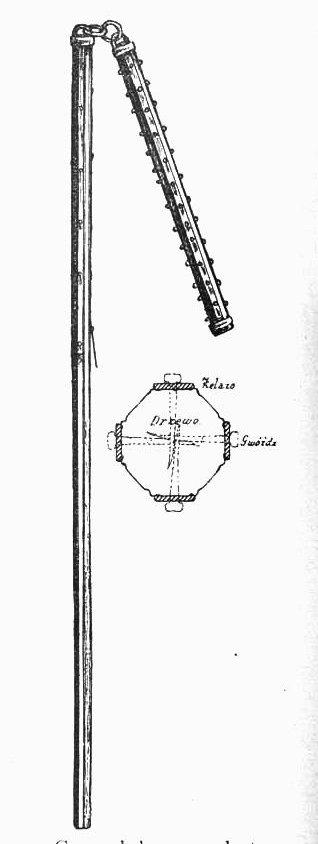
\includegraphics[height=5cm]{cep.jpg}
\end{figure}

\pagebreak
\section*{Rozdanie 23}
\handdiagramv{\vhand{T83}{KJ762}{854}{97}}
{\vhand{AK652}{T5}{T62}{A86}}
{\vhand{QJ974}{93}{AKQ93}{Q}}
{\vhand{}{AQ84}{J7}{KJT5432}}
{NSEW}

\begin{table}[h!]
    \centering
    \begin{tabular}{cccc}
        \vul{W} (B) & \vul{N} & \vul{E} (K) & \vul{S}\\
        -- & -- & -- & 1\spades \\
        2\clubs & 2\spades & 2\nt & 4\spades \\
        4\nt & \pass & 5\clubs & \dbl \\
        all \pass & & & \\
    \end{tabular}
\end{table}

[KG] Po mojej stronie stołu było śmiesznie, nie mogłam sobie wyobrazić rąk przeciwników.
2\nt było jakieś naturalne, inwitujące, w sumie ucieszyłabym się grając 2 (albo 3) \nt.
Na 4\nt też prawie spasowałam, ale ja bym to musiała grać. Myślałam, że 4\nt to młode,
ale i tak uważam, że się dogadaliśmy.\\
Wist 8\spades


[BS] Skok \vul{S} w końcówkę wywołał niemałą konsternację przy stole. Musi mieć jakiś potężny układ, może 6-5 z renonsem trefl?
Dużo wskazuje, że Krysia mogłą sobie ubzdurać, że 2NT to cośtam z czerwonymi. Bałem się dać 5\clubs, a 4NT jest dobrym 
zabezpieczeniem. 

[KK] Pasowałbym na 2\spades i się jarał. Ale jak już Cię 
zaswędziała dupa to 2\nt nat nie ma 
absolutnie żadnego sensu, musi być jakimś 
wariantem z fitem zwłaszcza, że 3\clubs to przepych.  

\pagebreak
\section*{Rozdanie 24}
\handdiagramv{\vhand{QJ}{J3}{AQ432}{JT98}}
{\vhand{KT96}{AK75}{KJ8}{K2}}
{\vhand{83}{Q8642}{6}{Q7654}}
{\vhand{A7542}{T9}{T975}{A3}}
{}

\begin{table}[h!]
    \centering
    \begin{tabular}{cccc}
        \nvul{W} (B) & \nvul{N} & \nvul{E} (K) & \nvul{S}\\
        \pass & 1\diams & 1\nt & \pass \\
        2\hearts & \pass & 3\spades & \pass \\
        4\spades & all \pass & & \\
    \end{tabular}
\end{table}

[KG] Wist 6\diams, oddane A\diams i przebitka.


\pagebreak
\section*{Rozdanie 25}
\handdiagramv{\vhand{AQ852}{A7}{T52}{754}}
{\vhand{T9}{KT643}{K43}{K92}}
{\vhand{J4}{95}{AQJ986}{AJT}}
{\vhand{K763}{QJ82}{7}{Q863}}
{EW}

\begin{table}[h!]
    \centering
    \begin{tabular}{cccc}
        \vul{W} (B) & \nvul{N} & \vul{E} (K) & \nvul{S}\\
        -- & \pass & \pass & 3\diams \\
        all \pass & & & \\
    \end{tabular}
\end{table}

[KG] Wist 2\spades\\
Nie no, gość miał 13, dyskusyjne to otwarcie.

[BS] ++ myślałem że miał 12.

[KK] Nie otwieramy.

\pagebreak
\section*{Rozdanie 26}
\handdiagramv{\vhand{K6}{QT654}{A95}{QJ6}}
{\vhand{AJ73}{J9872}{2}{T94}}
{\vhand{QT852}{A3}{KJ843}{A}}
{\vhand{94}{K}{QT76}{K87532}}
{NSEW}

\begin{table}[h!]
    \centering
    \begin{tabular}{cccc}
        \vul{W} (B) & \vul{N} & \vul{E} (K) & \vul{S}\\
        -- & -- & \pass & 1\spades \\
        \pass & 2\hearts & \pass & 3\diams \\
        \pass & 3\nt & all \pass & \\
    \end{tabular}
\end{table}

[BS] Wist 9\clubs. Zagrany pik do K i A, następnie trefl. Zabiłem Królem (mam wszystkie dojścia), zagrałem trefla.

Trochę gdybanie. Ale może lepiej przepuścić? Skąd rozgrywający ma widzieć, kto ma trefle? 
Zabicie bardzo sugeruje posiadanie \xdiams QT. Zresztą, \vul{N} odrzucając impas karo wygrywa!


[KG] Wpisane na złą linię :(

[KK] Ja bym zabił, może ma \xhearts AJ i jakiś squeeze 
się ustawi. A i tak masz dojścia.

\pagebreak
\section*{Rozdanie 27}
\handdiagramv{\vhand{Q743}{2}{AQ9532}{AT}}
{\vhand{62}{873}{J64}{98653}}
{\vhand{AT5}{KJ954}{T}{J742}}
{\vhand{KJ98}{AQT6}{K87}{KQ}}
{}

\begin{table}[h!]
    \centering
    \begin{tabular}{cccc}
        \nvul{W} (B) & \nvul{N} & \nvul{E} (K) & \nvul{S}\\
        -- & -- & -- & \alrts{2\diams} \\
        2\nt & all \pass & & \\
    \end{tabular}
\end{table}

[BS] Wist 5\diams wzięty waletem (1). Skoro mam mniej pików, to na pewno ma je \nvul{S}, prawda? 
Zagrałem kiera, w trakcie czego \nvul{N} wyciągnął kartę z ręki, więc położyłem \xhearts T, która wzięła (2).
No dobra, teraz to już na 100\% ma piki.
Zgrywam \xclubs KQ (3), \nvul{N} bije drugiego i gra pika do Asa, \nvul{N} odgrywa pika którego biję Królem (4).

O zgrozo, \nvul{N} dokłada! Dopiero teraz przypomniałem sobie otwarcie 3\diams Giorgi'a i ogarnąłem, że on umie w bloki.
Rozliczam rozdanie raz jeszcze i gram \xspades 9, licząc na wpust karowy.
\nvul{N} bije i gra pika do mojej blotki (5).

To umożliwia mi drugą próbę wpustu. Oddaję \xhearts 6 do \xhearts 9. S musi teraz dać mi dostęp do trefli lub lewę kierową, co czyni. (6, 7).
Noga. Ale z jaką historią!

[KK] Ale jak \xhearts T wzięła to założyłeś już, 
że ma kiery co nie? Tam źle Ci się napisało? 
Ma mieć piki i \xhearts KJ?\\
Bartoshu, nadajesz się do pisania artykułów do 
świata brydża. 

\end{document}